%%%%%%%%%%%%%%%%%%%%%%%%%%%%%%%%%%%%%%%%%%%%%%%%%%%%%%%%%%%%%%%%%%%%%%%%%%%%%%%%
% strategy: overview of analysis strategy
%%%%%%%%%%%%%%%%%%%%%%%%%%%%%%%%%%%%%%%%%%%%%%%%%%%%%%%%%%%%%%%%%%%%%%%%%%%%%%%%
\chapter{Analysis Strategy}
\label{ch:strategy}
The goal of this chapter is to provide an overview of the strategy adopted by this analysis. %The history of particle physics, the \CMS experiment at the \LHC, and cutting edge techniques in boosted-object physics have all been discussed. 
This analysis performs a direct search for LRS physics with a higher integrated luminosity than ever before, and uses boosted-object reconstruction techniques in an orthogonal selection region in order to search for LRS physics in an expanded \WRNR mass phase-space.

\section{Overview}

At this point, it is valuable to return attention to the Feynman diagram illustrating the \WRNR production and decay, Fig.~\ref{fig:mainDiag2}.
\begin{figure}[!tp]
    \centering
    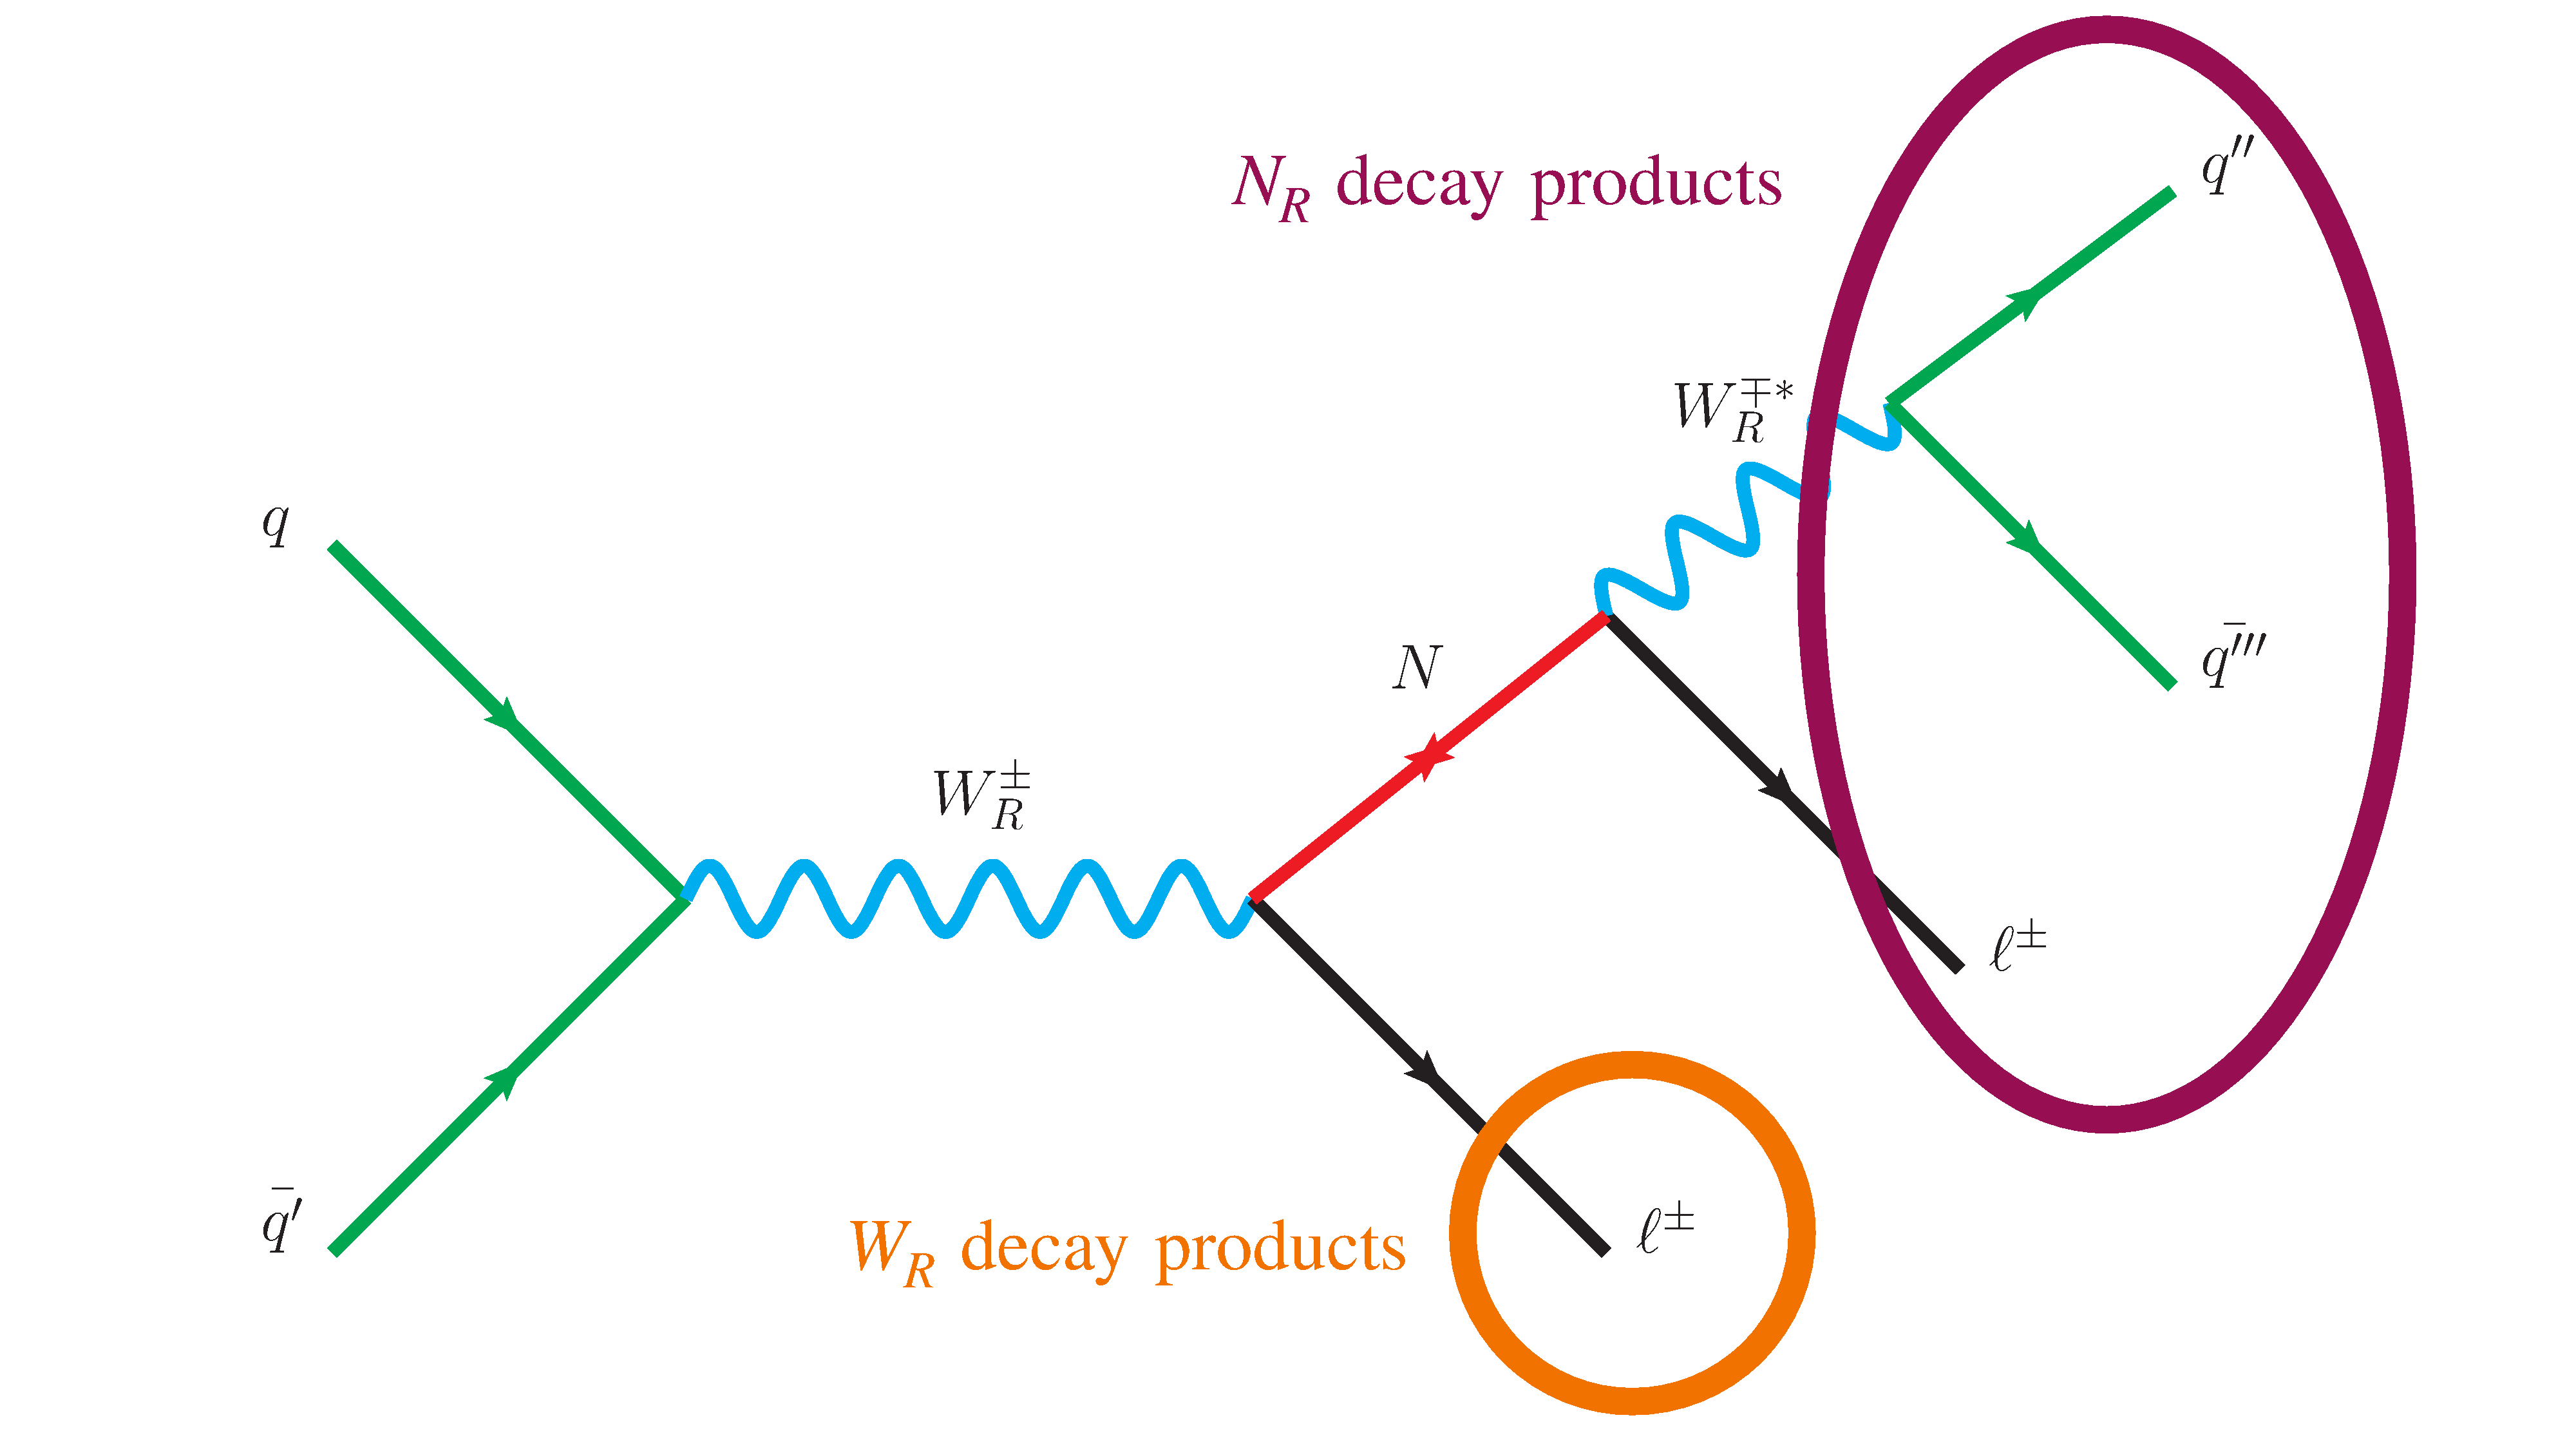
\includegraphics[width=\textwidth]{figures/labelledWRfeynman.pdf}
    \caption[
        \WR-\NR 4-object decay.
    ]{
      The principal Feynman diagram for this analysis.  Two quarks annihilate into a \WR boson, which decays to a lepton and a right-handed neutrino. This neutrino decays by a virtual \WR and another lepton.  This virtual boson decays to quarks, which produce jets. The final state objects produced from the \WR and \NR decay are highlighted separately. The relative separation of the \NR decay products from the \WR decay products changes in the \WRNR mass space.
    }
    \label{fig:mainDiag2}
\end{figure}
While the primary decay mode of a \WR would be a back-to-back quark-antiquark pair, as discussed in Section~\ref{sec:LRStheory}, searching for the leptonic decay of the \WR is more statistically powerful. However, the separation of the four decay objects is heavily dependent on the \NR mass. For a \NR mass substantially lighter than the \WR mass, the \NR decay particles collimate in the lab frame, boosted by the momentum of the \NR. The lepton produced in the initial \WR decay process will generally travel opposite to the \NR path, as the \WR will typically not be produced with significant momentum. 

Past analyses have required all four final-state objects to be well-separated in the lab frame \cite{EXO-17-011}, which relies on an increasingly-narrow kinematic phase-space as the \NR becomes lighter relative to the \WR. Some new selection criteria must be integrated into the analysis to pursue the lighter \NR phase-space. 

For this analysis, the strategy is to consider every \WRNR hypothesis with two orthogonal selections. 
%As most mass points will have a degree to which individual evens will pass one or both selection criteria, the selections are constructed to be orthogonal on a per-event level.
As no event can pass both selections, the total number of events passing each selection can be combined in the statistical analysis. In addition, the simple kinematic definition of the selection regions allows future theorists to cleanly reinterpret the results for new theories.

\section{Kinematic Region Selection}
The two signal regions will be discussed, starting with the lepton selection which is common to both signal regions. For an event which passes the lepton selection, the jets reconstructed in the event are evaluated with resolved selection. If this fails, the boosted selection is tried. The combination of the resolved and the boosted selections is designed to allow almost all signal events.

%Every event selection begins with the identification of leptons and \antikt size 0.4 jets. All of these objects must also pass kinematic requirements which ensure association with a hard process. If two highest transverse momentum leptons and jets are well separated, the event is identified as being resolved. If these objects are not well separated, or fewer than two size 0.4 jets are identified, the leptons are associated with jets reconstructed with a 0.8 size in the event. If there is a 0.8 size jet close to one of the leptons, and the other lepton is sufficiently far from it, the event is identified as boosted. Dividing events in this way does not rely on measuring the boost of the \NR and can be performed easily at a ``truth'' level to understand its behaviour fully with generated signal events.

%While a simple strategy would be to only search for a relatively heavier \NR masses with a resolved selection and create a new selection used exclusively for the relatively lighter \NR mass region, this technique struggles in an intermediate region, where the \NR decay objects are not guaranteed to be well resolved, or particularly collimated. 



\subsection{Lepton Selection}
Both types of signal selection require two well-separated leptons of significant transverse momentum. The leading lepton in the event must satisfy $\pt > \SI{60}{\GeV}$ and the sub-leading lepton must satisfy $\pt > \SI{53}{\GeV}$. These two leptons must also be separated by $\deltaR > 0.4$. 
%These two requirements remove a significant quantity of backgrounds both by number of events and variety of processes.
After these requirements, the dominant backgrounds are those with two real leptons, such as \Ztoee and \ttbar. General QCD processes and inclusive W processes are highly suppressed.
In addition, to keep the leptons within the tracker, and muon chamber acceptance, both leptons must satisfy $|\eta|<2.4$. This requirement reduces signal as well as background to some extent. Depending on the mass of the \WR, between $70-85\%$ of signal events pass these requirements at the generator level.

\subsection{Jet Selection}

\subsubsection{Resolved Approach}
The resolved jet selection begins by requiring at least two \antikt size 0.4 jets with a transverse momentum higher than $\SI{40}{\GeV}$. Requiring this momentum from the jets reduces background and helps guarantee that the jets did in fact come from a hard-process (more about this will be discussed in Chapter~\ref{ch:objs}). The jets are also required to have their center-of-momentum within $|\eta|$ of $2.4$. This requirement mimics the $\eta$ requirement placed on the leptons. These jets also must be more than 0.4 in $\deltaR$ apart from each other and the two selected leptons. This multi-object separation requirement ensures that this event can be reconstructed under a resolved paradigm. If events fail to identify the two jets, or they are not sufficiently separated, the boosted selection is attempted.

\subsubsection{Boosted Approach}
The boosted jet selection begins by requiring events to have at least one \antikt size 0.8 jet with a transverse momentum higher than $\SI{200}{\GeV}$. In a signal event, the \NR jet will have a large amount of momentum, and so this requirement is not significantly penalizing. This gives a great opportunity to remove significant amounts of background. For the same reason as the resolved selection, the fat jet must have an $|\eta|<2.4$. 

The next boosted jet requirement is that the sub-leading lepton must fall within the cone of the fat jet. This requirement ensures that the fat jet selected is \NR-jet like. In addition, while \CMS produces jets in abundance, even at these high transverse momenta, high transverse momentum leptons are uncommon within these jets. To guarantee that not only is the sub-leading lepton within the jet, but also that the leading lepton travels away from the \NR jet, the $\Delta\phi$ between the fat jet and the leading lepton must be at least $2.0$.

\subsection{Multi-Object Selections}

Having selected all of the jets and leptons necessary to reconstruct the event under either the resolved or boosted paradigm, the qualities of combinations of these objects can now be judged. 
\subsubsection{\WR Mass}
This analysis hopes to reconstruct the \WR mass peak. In the resolved case, this is done by summing the 4-vectors of the four selected objects and calculating the mass of that sum; $M_{\ell\ell jj}$. In the boosted paradigm, the \WR mass can be reconstructed from the \NR jet ($J$) and the leading lepton ($\ell$); $M_{\ell J}$. 
As this analysis focuses on extending the limit of past analysis in the \WRNR mass phase-space, the requirement on the \WR mass can be placed quite high to obliterate remaining background rates. In both analyses, the reconstructed \WR mass must be at least $\SI{800}{\GeV}$.
The shape of four different \WR masses, spread across the searched region are shown in Fig.~\ref{fig:truth_sig_eff}.

\begin{figure}[!tp]
 \centering
    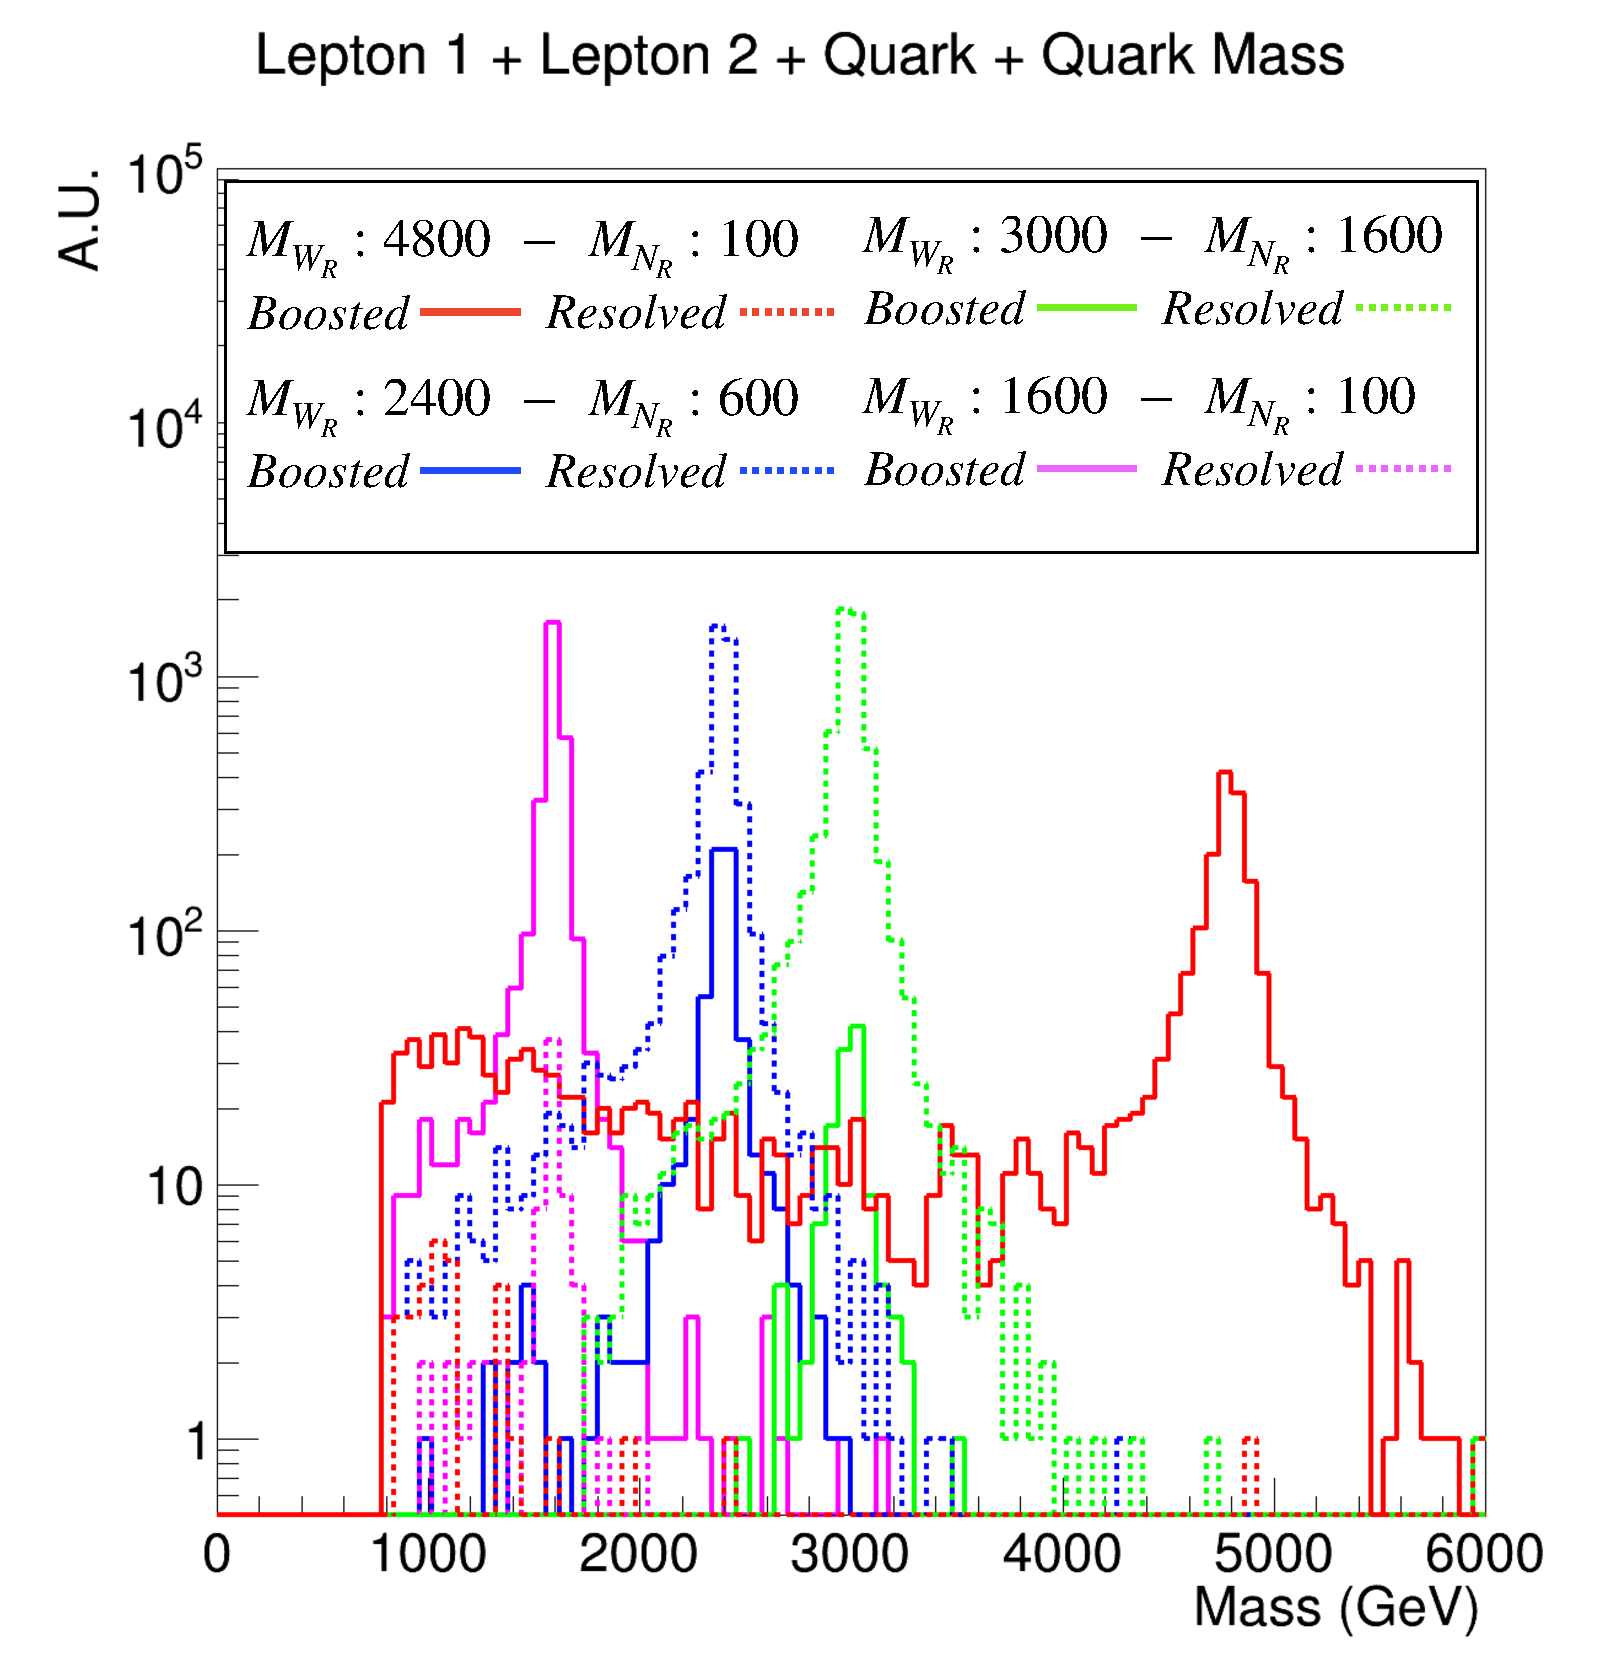
\includegraphics[width=\textwidth]{figures/LLQQ_mass.pdf}
    \caption[
        %Short caption for the list of figures
       Generated \WR spectra.
    ]{
        % Full caption shown below the image
       
        The \WR mass for four different \WR and \NR mass hypotheses. The integral of each histogram is scaled relative to the acceptance of the analysis at that mass point. The resolved selections are shown with dashed lines, and the boosted selections are shown with solid lines. It can be seen that for the most massive and most boosted mass point, the boosted selection far outperforms the resolved selection, which only succeeds in the lower off-shell tail of the \WR spectrum. The shape of this spectrum is discussed in Section~\ref{sec:WRshape}.
       
    }
    % A label so you can \ref{fig:my_fig}. It is arbitrary; neither the 'fig:'
    % nor the fact that it has the same name as the pdf are required.
    \label{fig:truth_sig_eff}
\end{figure}


\subsubsection{Di-lepton Mass}
\label{sec:DYSB}
One of the most significant backgrounds in this analysis comes from the Drell-Yan process. Off-shell high-mass Drell-Yan events and high-momentum, mis-reconstructed Drell-Yan both form parts of this background for both boosted and resolved selection regions. To significantly reduce this background, a requirement is placed on the mass of di-object formed by the two selected leptons. This mass must be higher than $\SI{400}{\GeV}$.

In past analyses, the di-lepton mass requirement was considerably lower, at $\SI{200}{\GeV}$. While this requirement is certainly high enough to drastically reduce the on-shell Drell-Yan background, it was increased to further reduce all backgrounds for this analysis. A comparison of the expected limits for across \WR masses for the new ($\SI{400}{\GeV}$) and old ($\SI{200}{\GeV}$) requirements for the resolved analysis is shown in Fig.~\ref{fig:mll_comparison}. Generally, the expected limit is improved by $10-20\%$ for \WR masses higher than $\SI{1000}{\GeV}$.

\begin{figure}[!tp]
    \centering
    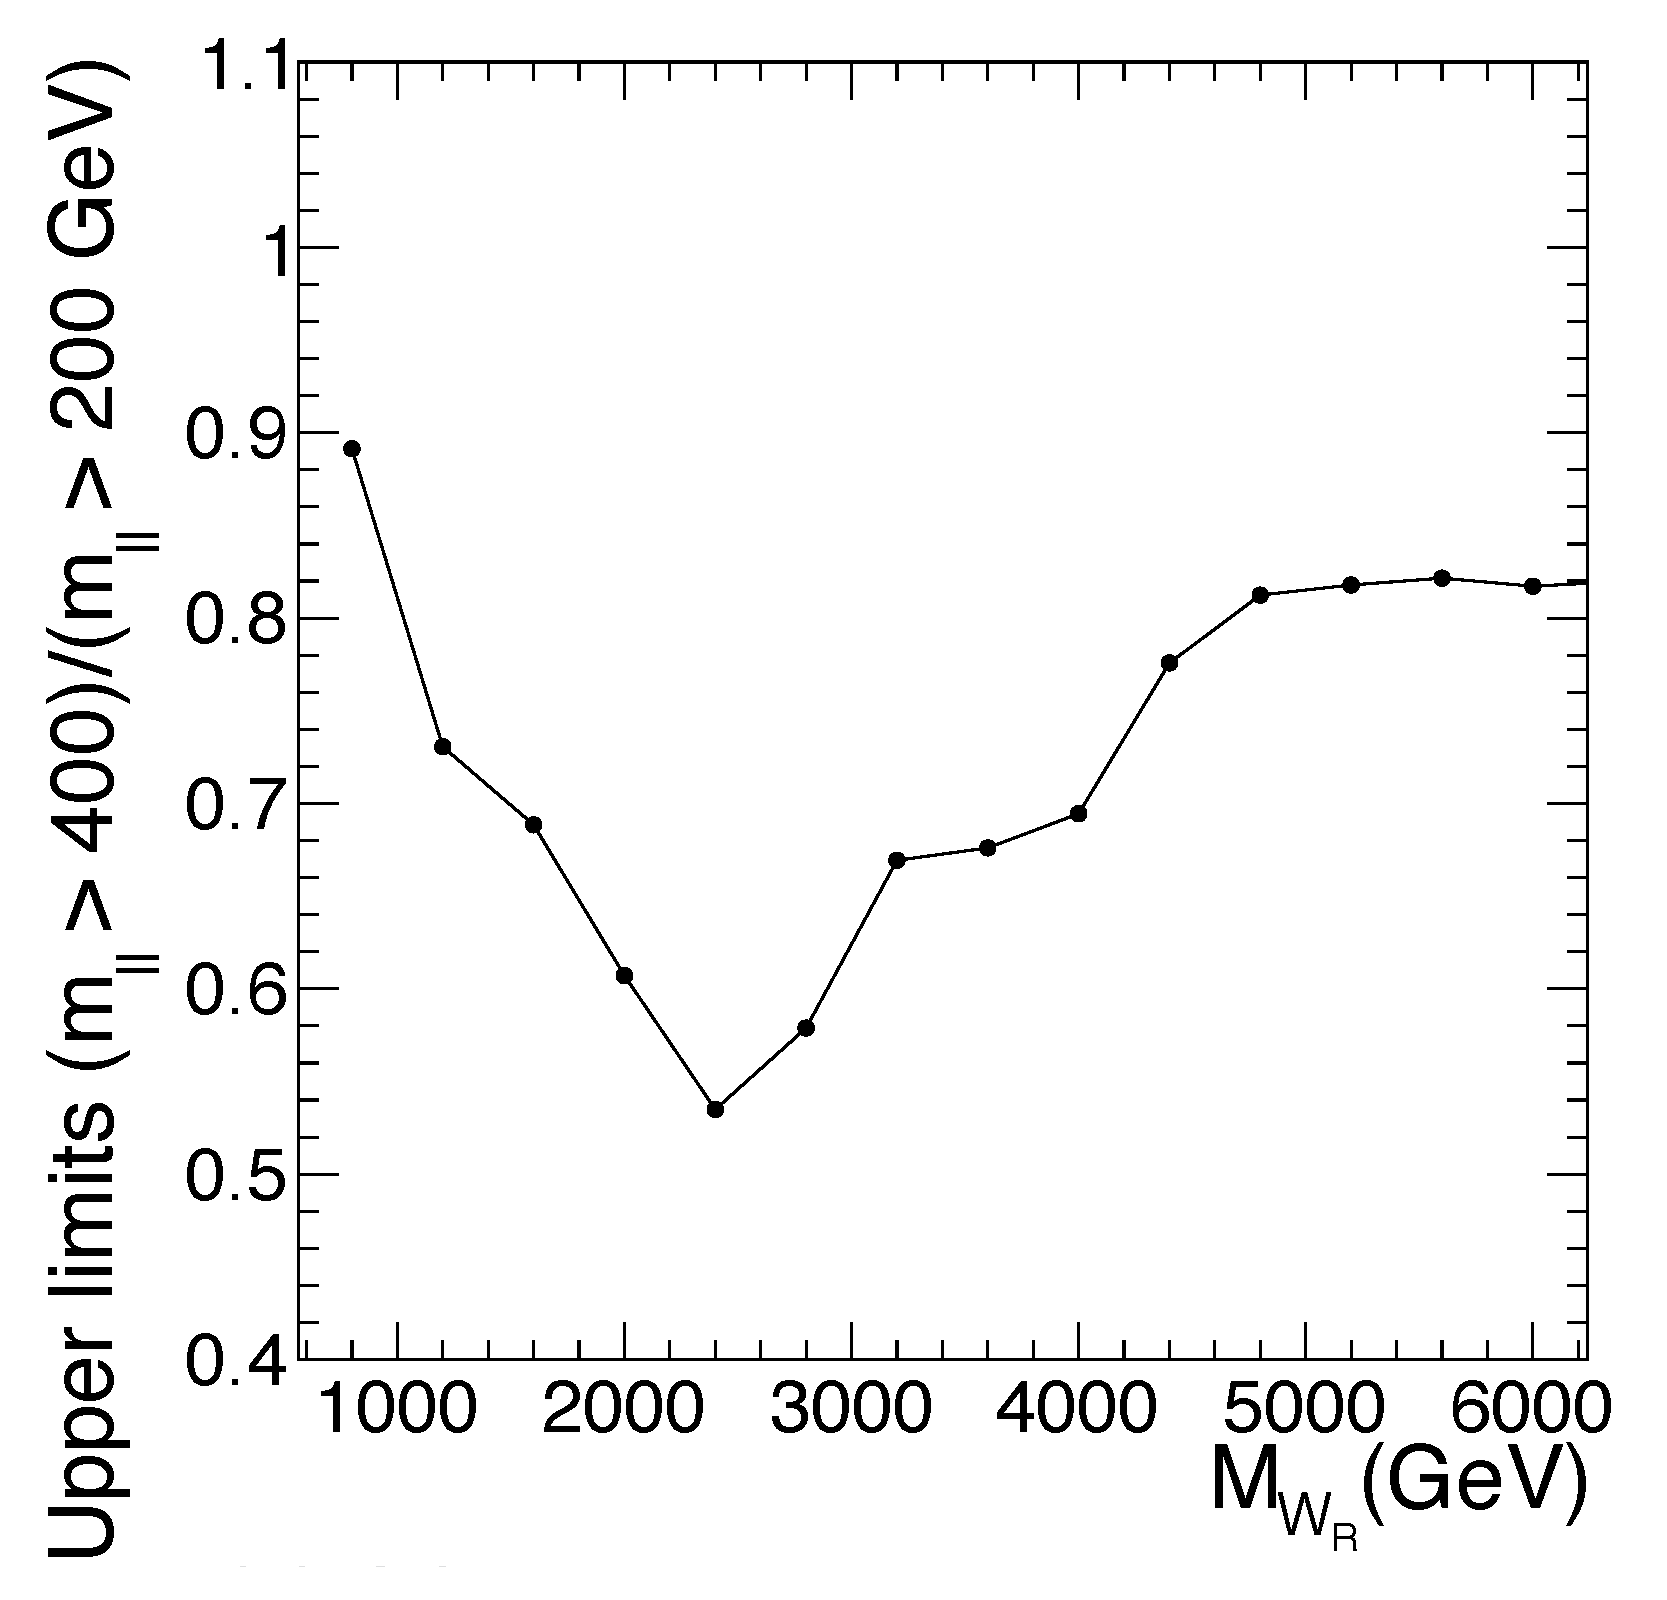
\includegraphics[width=\textwidth]{figures/Mll200vs400.pdf}
    \caption[
      Limit performance versus $M_{\ell\ell}$
    ]{
      The ratio of the expected limits in the muon channel of the resolved analysis with the $M_{\ell\ell} > \SI{400}{\GeV}$ and $M_{\ell\ell} > \SI{200}{\GeV}$. The expected limits are calculated for signals with $M_{\WR}/M_{\NR} = 2$. The expected limits are stronger for the $M_{\ell\ell} > \SI{400}{\GeV}$ selection for all signals with $M_{\WR}>\SI{1000}{\GeV}$.
    }
    \label{fig:mll_comparison}
\end{figure}

\section{Lepton Flavor and Kinematic Sidebands}
In this analysis, the behavior of background and signal in the signal region are simulated. When data is studied in the signal region, the question is then posed whether the data behaves more consistently with background or a background + signal hypothesis. In order to understand the behaviour of background and signal without looking directly at the data (which would potentially contaminate the analysis), alternate selection regions are created to validate and correct simulated background behaviour. These regions are commonly called ``sidebands''. In this analysis, sidebands are created by changing two kinematic requirements, $M_{\ell\ell}$ and $M_{\ell\ell jj}/M_{\ell J}$ and the lepton flavor requirements are changed to create a signal-like (but signal-free) sideband. These requirement changes create, in total, four sidebands.

\subsection{Kinematic Sidebands}

\subsubsection{\WR Mass}
The shape of $M_{\ell\ell jj}/M_{\ell J}$ for all backgrounds in this analysis is expected to approximately exponentially fall before and through the signal region. Therefore, this background behaviour can be studied in a region with a reconstructed \WR mass of less than $\SI{800}{\GeV}$. This forms the low-mass sideband of the analysis.

\subsubsection{Di-lepton Mass}
To form a sideband where the behaviour of Drell-Yan can be studied, the $M_{\ell\ell}$ mass requirement is changed to be less than $\SI{200}{\GeV}$ in the resolved selection and $\SI{150}{\GeV}$ in the resolved selection. This allows resonant Drell-Yan events to be studied and their behaviour extrapolated to the signal region.

Forming the low di-lepton mass selection region requires the loosening of additional requirements in the boosted selection. The sub-leading lepton is no longer required to be within the fat-jet. Requiring the second lepton to be within the jet in the low mass region almost entirely depopulates the region, severely limiting what can be studied in it.

\subsection{Flavor Sideband}
This analysis focuses on two lepton flavors, muon and electron. While, generally, any LRS extension would apply to all lepton flavors, the tau flavor is not searched for, as it poses several different, unique challenges \cite{wprimetotau}. Likewise, LRSM theories do not preference a right-handed neutrino mass-hierarchy. Therefore, there is no reason to expect the right-handed tau neutrino to appear in a similarly searchable mass region as the two flavors searched for in this analysis.

As signal events will produce two same-flavor leptons, this analysis selects background events which contain one electron and one muon as well. This selection produces an almost completely signal-free flavor sideband where lepton-flavor independent backgrounds can be studied, the most significant of which is \ttbar. While the low $M_{\ell\ell}$ region is dominated by Drell-Yan events, these events are unlikely to appear in the flavor sideband (as the Z boson produces same flavor leptons), unless the Z decays to the tau, and these independently to two different leptons. The Z decay to leptonically-decaying taus occurs at a much lower rate, however, than the second dominant background. A \ttbar event has two independent W boson decays in its decay process. This means \ttbar can be studied thoroughly in both data and Monte-Carlo in this region. The flavor sideband also spans two kinematic selection regions, the low and high $M_{\ell J} - M_{\ell \ell j j}$ mass regions. A diagram of the four regions produced is shown in \ref{fig:selection_regions}.
\begin{figure}[!tp]
    \centering
    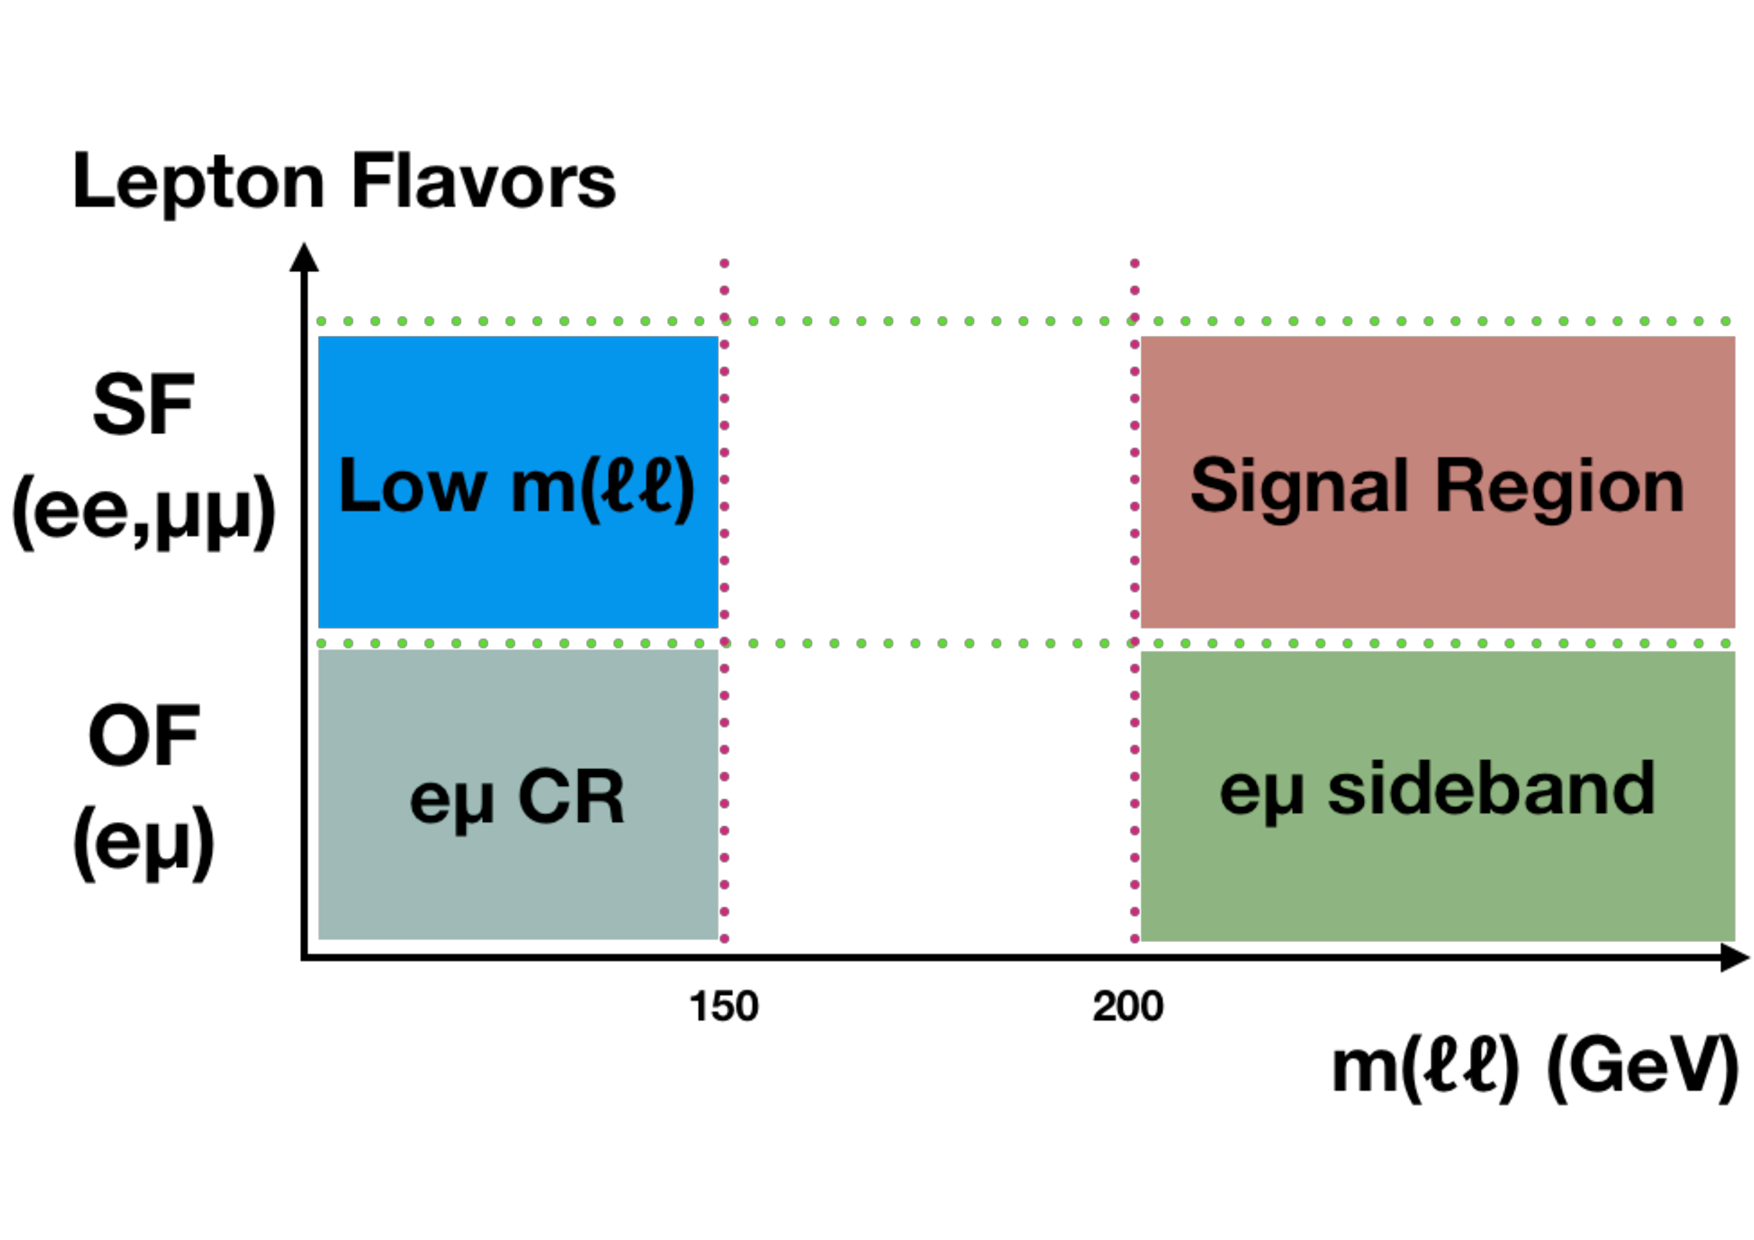
\includegraphics[width=\textwidth]{figures/Schem.pdf}
    \caption[
        %Short caption for the list of figures
       Analysis control regions.
    ]{
        % Full caption shown below the image
       The multi-object mass and lepton flavor permutation are used to create four selection regions. This allows for the \ttbar behaviour to be studied in both data and MC in the signal mass regime.
       
    }
    % A label so you can \ref{fig:my_fig}. It is arbitrary; neither the 'fig:'
    % nor the fact that it has the same name as the pdf are required.
    \label{fig:selection_regions}
\end{figure}


%\begin{description}
%\item[Individual Object Selection:] \
%  \begin{itemize}
%  \item leading \pt lepton with $\pt > \SI{60}{\GeV}$
%  \item sub-leading \pt lepton with $\pt > \SI{53}{\GeV}$
%  \item at least two AK4 jets with  $\pt > \SI{40}{\GeV}$
%  \item all leptons and jets with $|\eta| < 2.4$
%  \item all objects $\Delta R > 0.4$ apart
%  \end{itemize}
%\item[Multi-object Selection:]\
% \begin{itemize}
%  \item di-lepton mass $m_{\ell\ell} > \SI{400} {\GeV}$: to suppress %DY+jets contribution
%  \item $M_{\ell \ell j j} > \SI{800}{\GeV}$
%  \end{itemize}%
%
%\end{description}

%The individual object \pt selections serve to remove background events and safely exceed trigger requirements which are covered in Chapter~\ref{ch:objs}. The $\eta$ requirements are likewise very efficient with \WR events because the very heavy \WR is very unlikely to be produced with significant longitudinal momentum. The requirement itself keeps all of the objects within the highest performance regions of \CMS. The key requirement for separating this selection from boosted events, is that each object must be isolated from the others, achieved with a $\deltaR$ between all objects to be larger than the jet size.

%The multi-object selections serve to produce two control regions and reduce backgrounds. The low-mass control region is defined as having a four-object mass of less than any expected signal. This region has far more background events. The behaviour of the background in this region is expected to be the same as its behavior as the four-object mass increases, allowing for a check of the background estimation. The di-lepton mass selection does not significantly change the signal acceptance fraction. For Drell-Yan, however, a large di-lepton mass can only come from mis-reconstruction or very off-shell Drell-Yan production. Separating out on-shell Drell-Yan reduces the background noticeably, and gives a region where the background can be used to check the simulated di-lepton mass shape with data. The signal region selection is designed to exceed the Drell-Yan selection to prevent migration between selection regions. These two sidebands are selected as follows:

%\begin{description}
%\item[low $M_{\ell\ell jj}$ resolved control region:]\ 
%  \begin{itemize}
%  \item same as resolved signal region, but $M_{\ell \ell j j} < \SI{800}{\GeV}$
%  \item di-lepton mass $m_{\ell\ell} < \SI{200}{\GeV}$
%  \end{itemize}
%\end{description}



%\begin{description}
%\item[low $M_{\ell\ell}$ resolved control region:]\ 
%  \begin{itemize}
%  \item same as resolved signal region, but item di-lepton mass %$\SI{60}{\GeV} < m_{\ell\ell} < \SI{150}{\GeV}$
%  \end{itemize}
%\end{description}
%The efficiency of the kinematic component of the resolved selection is shown for a variety of different mass points.

%\subsection{Boosted Signal Kinematic Selection}

%In this case, jets reconstructed with a large size, $R=0.8$ are used, called ``fat'' jets. These fat jets are selected to have significant \pt as \NR jet produced in a signal event is expected to have significant transverse momentum. Two kinematic sideband regions are used for the boosted selection as well, and these are very similar to the resolved sideband selections. The Drell-Yan control region is defined just as it is for the resolved selection, using the invariant mass of the two leptons. For the boosted control region, sub-leading lepton is not required to be within the jet, or for the LSF to be any value. Both of these requirements would effectively empty the Drell-Yan sideband. The low-mass sideband is defined with the mass of the leading lepton and fat-jet di-object, as this di-object is used to profile the \WR mass.

%\begin{description}
%\item[Boosted signal region:] \
%  \begin{itemize}
%  
%  \item leading lepton with $\pt > \SI{60}{\GeV}$
%  \item sub-leading lepton with $\pt >\SI{53}{\GeV}$
%  \item at least one AK8 jet with  $\pt >\SI{200}{\GeV}$
%  \item the sub-leading lepton must fall within the cone of the AK8 jet
%  \item all leptons and jets with $|\eta| < 2.4$
%  \item di-lepton mass $m_{\ell\ell} > \SI{400}{\GeV}$
%  \item $\Delta \phi > 2.0$ between selected jet and lead lepton
%  \item $M_{\ell J} > \SI{800}{\GeV}$
%  \end{itemize}
%\end{description}

%\begin{description}
%\item[low $M_{\ell J}$ boosted control region:]\ 
%  \begin{itemize}
%  \item same as boosted signal region, but $M_{\ell j} < \SI{800}{\GeV}$
%  \end{itemize}
%\end{description}

%\todo{background distributions in these two sideband regions}

%\begin{description}
%\item[low $M_{\ell\ell}$ boosted control region:]\ 
%  \begin{itemize}
%  \item same as boosted signal region, but
%  \item di-lepton mass $m_{\ell\ell} < \SI{150}{\GeV}$
%  \item no LSF requirement on AK8 jet
%  \item no requirement that sub-leading lepton be contained within the %AK8 jet
%  \end{itemize}
%\end{description}


%-CAN ALSO DEFINE CROSS-CHANNELS HERE
%-HUGE SELECTION LIST IS HORRIBLE
%-ANYTHING THAT CAN BE APPLIED AT GENERATOR LEVEL CAN BE PART OF THE STRATEGY -- IGNORES HEEP ETC... REALITY
%-WE'RE LOOKING DEFINE THESE REGIONS, SO WE ASK FOR ENERGETIC LEPTONS IN THE DETECTOR BECAUSE WE WANT SOMETHING HEAVY
%-ABSORB EVENT SELECTION, PRECEDE OBJECT ID
%-ADD TRIGGER TO OBJECT ID
%-TRIGGER POINT: FOR OUR EVENTS WE HAVE TWO MUONS SO IT'S EVEN MORE EFFICIENT
%-WHAT ARE TYPICAL EFFICIENCIES FOR A SELECTION OF MASSES?  WHAT IS DENOMINATOR IN OUR PLOTS?
%-WHAT IS THE ACCEPTANCE HIT AFTER SELECTION
%-CAN DROP NON PHYSICSY CORRECTIONS
%-WHAT IS THE ID HIT TO ACCEPTANCE?  DENOMINATOR: GEN ACCEPTED
%-DISCUSSION OF BOOSTED SIGNAL SHAPE COULD BE TACKED ON EARLIER (TO LIKE PDFS FOR EXAMPLE) THERE'S ALWAYS A HIGH MASS EFFECT FOR SOME EVENTS. OFF-RESONANCE PRODUCTION IS TRUNCATED BY NR MASS MAYBE IN CHAPTER 2  sdf 
